\section{Documenti}
Tutti i documenti gestiti dalla piattaforma TURING sono astratti dalla classe \textbf{Document}, che mantiene i riferimenti alle singole sezioni, a loro volta rappresentate dalle istanze della classe \textbf{Section}. Come illustrato dal class diagram \ref{fig:document_class_diagram}, il documento si occupa di mantenere i riferimenti agli utenti aventi i permessi di accesso al contenuto delle singole sezioni\footnote{Vengono mantenuti i riferimenti sia al profilo del creatore del documento, sia alla lista di coloro i quali hanno accesso alla struttura come \textit{modifiers}. In questo modo, il sistema è in grado di negare la possibilità a questi ultimi di aggiungere altri utenti alla lista degli aventi accesso, lasciando questa possibilità unicamente ai creatori, come da specifiche.}.

Tutte le operazioni su filesystem relative alla \underline{gestione dei documenti} sono effettuate \underline{tramite NIO}.
\paragraph{Accesso Esclusivo}
La gestione dell'accesso esclusivo al contenuto delle sezioni viene lasciata agli oggetti \textbf{Section}, che mantengono tra le proprietà d'istanza una \textbf{Lock}\footnote{Si è scelto di utilizzare un oggetto di tipo \textbf{ReentrantLock}.}, la quale viene utilizzata per l'accesso alle sezioni critiche relative all'assegnazione dei riferimenti dell'utente che è in \textit{Editing Mode}. Per comprendere, infatti, se esiste già o meno un utente in questa fase sulla sezione obiettivo, si analizza la variabile \textbf{userOnEditing} e, se questa è \textit{null}, allora si procede all'assegnazione del riferimento dell'utente richiedente.

\begin{figure}[h]
	\caption{Schema di rappresentazione delle stringhe}
	\label{fig:document_class_diagram}
	\centering
	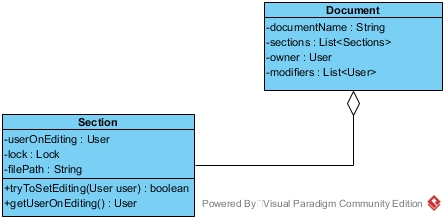
\includegraphics[scale=0.7]{assets/document_class_diagram.jpg}
\end{figure}

\paragraph{Memorizzazione Locale}
A livello fisico ogni documento è una vera e propria directory, mentre le sezioni sono file al suo interno. Al momento della creazione di un nuovo documento, vengono generate le sezioni aventi un filename randomico\footnote{Si è scelto di utilizzare il valore del timestamp misurato al momento della creazione della prima sezione e successivamente incrementato di uno per ognuna delle restanti.}. Sarà poi l'oggetto \textbf{DocumentsDatabase} ad occuparsi di mantenere i riferimenti alla lista completa dei documenti\footnote{In realtà, si sfrutta una struttura \textit{factory} per la generazione dei documenti: non viene mai creato un \textbf{Document} utilizzando il suo costruttore, ma si sfrutta il metodo \textbf{createNewDocument} del \textbf{DocumentsDatabase}, che a cascata provocherà la generazione di documento e sezioni.} e ad interfacciarsi con il resto della piattaforma.